\documentclass[a4paper,12pt]{article}
\usepackage[utf8]{inputenc}
\usepackage[lmargin=3cm,tmargin=3cm,rmargin=2cm,bmargin=2cm]{geometry}
\usepackage[singlespacing]{setspace}
\usepackage[T1]{fontenc}
\usepackage[brazil]{babel}
\usepackage{graphicx,xcolor,comment,enumerate,multirow,multicol}
\usepackage{indentfirst}
\usepackage{amsmath,amsthm,amsfonts,amssymb,dsfont,mathtools,blindtext}
\usepackage{booktabs}
\usepackage{caption}
\usepackage{times}
\usepackage[alf]{abntex2cite}
\usepackage{hyperref} %% Referências com label, o site.
\usepackage{multirow} %% Diversas colunas, na tabela

\setlength{\parindent}{1.3cm}

\pagestyle{empty}

\begin{document}

\begin{table}[htb]
	\begin{center}
		\begin{tabular}{cc}
			\begin{tabular}{p{3.5cm}} 
\includegraphics[scale=0.075]{3} \end{tabular} &
			\begin{tabular}{c} \huge \bf Universidade de São Paulo \\ \\ \Large Escola de Engenharia de Lorena - EEL
			\end{tabular}
		\end{tabular}
	\end{center}
\end{table}

\vspace{1.5cm}

\begin{center}
	\Large{\bf Física experimental 3} \\
	\vspace{1.5cm}
	\large{Experimento 5: Mapeamento de superfícies equipotenciais} \\
	\vspace{2.0cm}
\end{center}

\vspace{4cm}

\large{\flushleft{\bf{Autor e N\textsuperscript{o} USP:}}
  \vspace{0.4cm} \\
  Vinicius Gabriel Gomes de Albuquerque, 11201742}
\vspace{3.0cm}

\begin{center}
	\textbf{Professor}: Fernando Catalani \\
	\vspace{3cm}
	Lorena - Junho de 2020
\end{center}

\newpage

\section*{Resultados e discussões}
A seguir estarão mostradas as figuras com as linhas equipotenciais de campo elétrico para condutores circulares e retos nas figuras \ref{fig:circular} e \ref{fig:reto}, respectivamente.

\begin{figure}[!h]
   \centering
   \caption{\label{fig:circular}Equipotenciais de condutores circulares}
   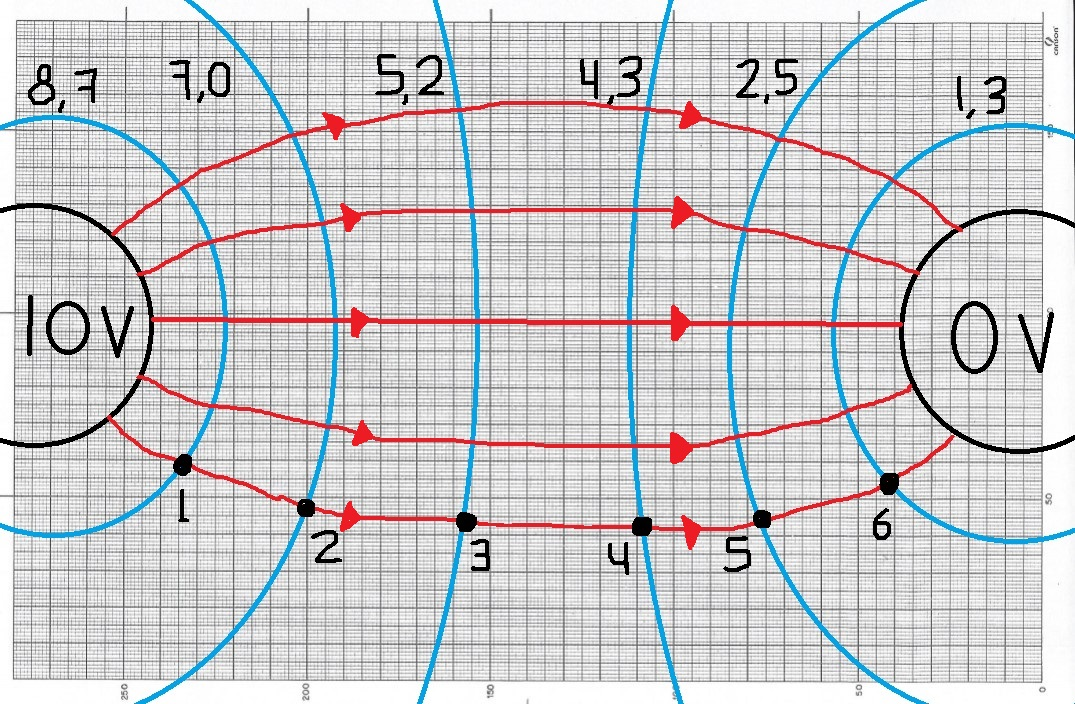
\includegraphics[scale=0.4]{1}
   \legend{Fonte: Autoria própria}
\end{figure}

\begin{figure}[!h]
   \centering
   \caption{\label{fig:reto}Equipotenciais de condutores retos}
   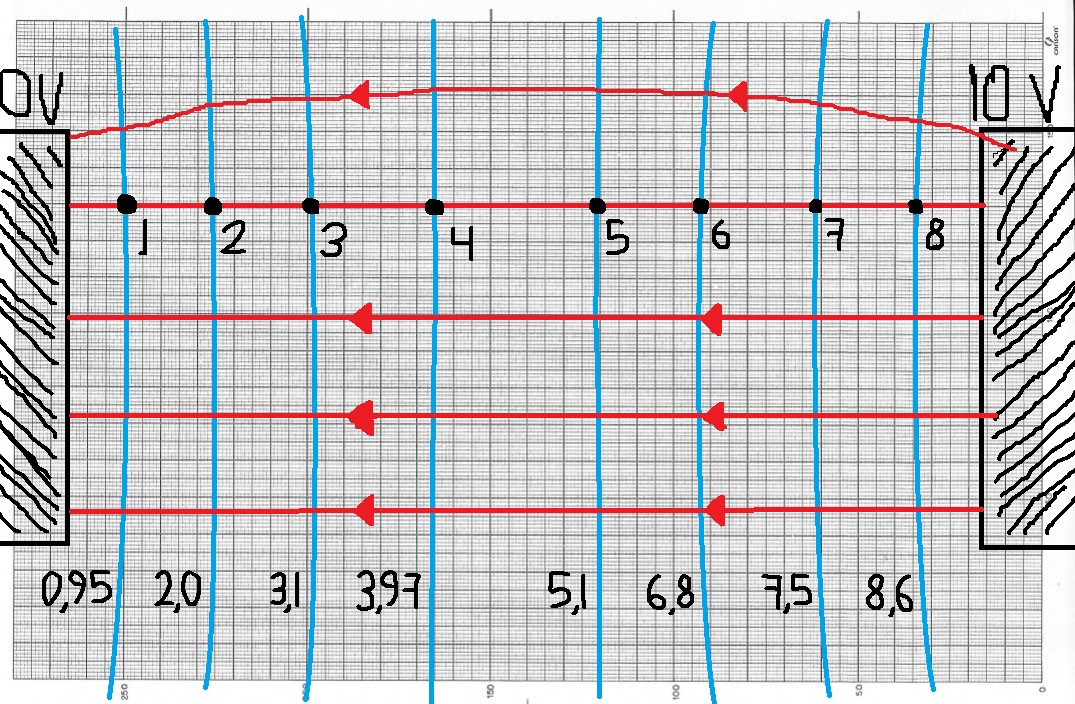
\includegraphics[scale=0.4]{2}
   \legend{Fonte: Autoria própria}
\end{figure}

Ambas as figuras mostradas anteriormente mostram algumas linhas de campo, que são perpendiculares às linha equipotenciais, os valores de potencial em todas as equipotenciais e alguns pontos, um em cada equipotencial, cuja intensidade de campo elétrico será calculada.

Os pontos marcados nas figuras \autoref{fig:circular} e \autoref{fig:reto} servem de referência, mas não representa a escala que será usada daqui em diante para fins de cálculo, agora serão utilizados os pontos fornecidos no roteiro do experimento. Os dados referentes ao condutor circular estão listados na \autoref{tab:circular} e os dados para o condutor reto na \autoref{tab:circular}.

\begin{table}[!h]
   \centering
   \caption{\label{tab:circular}Dados referentes à configuração dos condutores circulares}
   \begin{tabular}{lcccccc}
     \hline
      \multicolumn{7}{c}{\textbf{Ponto}} \\
     \midrule
     \midrule
      $\Delta V \, (\mathrm{V})$ & 1 & 2 & 3 & 4 & 5 & 6 \\
      \midrule
     $\Delta x \, (\mathrm{m})$ &&&&&& \\
     \hline
      $E \, (\mathrm{V/m})$ &&&&&& \\
      \bottomrule
   \end{tabular}
   \vspace{1.7mm}

   \legend{Fonte: O autor}
\end{table}



\end{document}
%%% Local Variables:
%%% mode: latex
%%% TeX-master: t
%%% End:
